% =========================================================== Q5
\section*{Q5: Mitigate Over-Smoothing in Deep GNNs (6 pts)}

\begin{lstlisting}[style=p1pystyle]
class MyDeepConv(MessagePassing):
    """APPNP-style decoupled propagation: transform once, then K personalised-PageRank
    steps. One layer reaches K hops, so K=8 gives an 8-hop receptive field at n_layers=1.
    """

    def __init__(self, in_channels, out_channels, K=8, alpha=0.3):
        super().__init__(aggr="add")
        self.in_channels = in_channels
        self.out_channels = out_channels
        self.K = K            # propagation steps = hops: K=8 at n_layers=1 is 8 hops
        self.alpha = alpha    # teleport probability, chosen on validation MRR
        self.lin1 = nn.Linear(in_channels, out_channels)
        self.lin2 = nn.Linear(out_channels, out_channels)
        self.reset_parameters()

    def reset_parameters(self):
        super().reset_parameters()
        self.lin1.reset_parameters()
        self.lin2.reset_parameters()

    def forward(self, x, edge_index):
        edge_index, _ = remove_self_loops(edge_index)
        edge_index, _ = add_self_loops(edge_index, num_nodes=x.size(0))
        src, dst = edge_index[0], edge_index[1]
        deg_inv_sqrt = degree(dst, x.size(0), dtype=x.dtype).pow(-0.5)
        norm = deg_inv_sqrt[src] * deg_inv_sqrt[dst]

        # Prediction first: all the parameters live here, none in the propagation,
        # so the hop count K is free of parameters and cannot overfit with depth.
        h = self.lin2(F.relu(self.lin1(x)))

        # Z <- (1 - alpha) A_hat Z + alpha H, K times: personalised PageRank with
        # restart to H, so the node's own features are re-injected at every hop.
        z = h
        for _ in range(self.K):
            z = (1 - self.alpha) * self.propagate(edge_index, x=z, norm=norm) \
                + self.alpha * h
        return z

    def message(self, x_j, norm):
        return norm.view(-1, 1) * x_j
\end{lstlisting}

\paragraph{Why stacking fails, and what this does instead.}
Li, Han and Wu~\cite{p1:li2018} identify the GCN propagation
$\hat D^{-1/2}\hat A\hat D^{-1/2}$ as a form of Laplacian smoothing and prove (their
Theorem~1) that repeating it drives every vertex in a connected component to the same
features, proportional to the square root of its degree. Their own remedy keeps the GCN
shallow and adds labels --- co-training with a random-walk model, and self-training ---
so it does not make deep propagation safe, which is what this question needs. I
implement instead the fix of Gasteiger, Bojchevski and G\"unnemann~\cite{p1:appnp}:
separate the \emph{prediction} from the \emph{propagation}. Theirs is personalised
PageRank, $Z \leftarrow (1-\alpha)\hat A Z + \alpha H$, re-injecting the node's own
transformed features at every step with teleport probability $\alpha$. An ordinary
$k$-step propagation instead converges to a limit that is ``independent of the random
walk's starting (root) node'' and so ``unsuitable for describing the root node's
neighborhood''; the teleport term is what keeps the operator anchored to the root.

\paragraph{Why this is 8 hops, and why \texttt{n\_layers=1}.}
One call to \texttt{propagate} moves information one hop, so a stack of $L$ layers each
propagating $K$ times has a receptive field of $L \times K$ hops. This layer runs $K=8$
steps inside a single \texttt{forward}, so $1 \times 8 = 8$ hops, and the Q5 cell is run
with \texttt{n\_layers=1}. Because the propagation holds no weights, that depth is free:
the model has $8{,}320$ parameters, identical to the 2-layer GCN and a quarter of the
8-layer GCN's $33{,}280$. $\alpha=0.3$ was chosen on validation MRR alone and sits on a
plateau (val MRR $0.733$--$0.737$ for $\alpha \in [0.25, 0.5]$, falling to $0.699$ at
$\alpha=0.2$); the original paper uses $\alpha=0.1$ with $K=10$.

\begin{figure}[H]
  \centering
  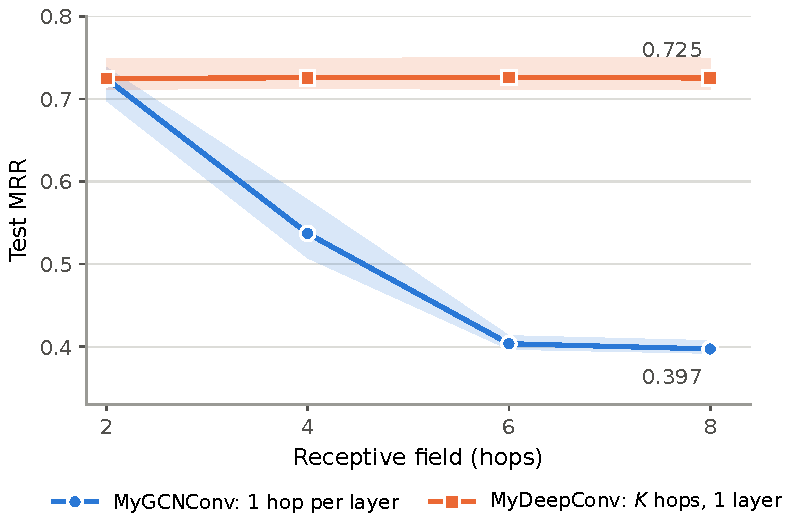
\includegraphics[width=0.78\linewidth]{fig_p1_depth.pdf}
  \caption{Test MRR against receptive-field depth. Each line is the mean over
  three node2vec draws; the shaded band is the min--max over those same three
  seeds.}
  \label{p1:fig:depth}
\end{figure}

\noindent
Stacking \texttt{MyGCNConv} to reach $8$ hops costs $45\%$ of its test MRR
($0.724 \to 0.397$, mean over three seeds), while \texttt{MyDeepConv} is flat to within
noise over the same range ($0.725, 0.725, 0.726, 0.725$ at $2, 4, 6, 8$ hops). The gain
is robustness to depth, not a better score: at $8$ hops \texttt{MyDeepConv} scores
$0.725$ against the $8$-layer GCN's $0.397$, but only matches the $2$-layer GCN, whose
three-seed mean of $0.724$ is indistinguishable from it.

\begin{table}[H]
  \centering
  \setlength{\tabcolsep}{4.5pt}% keep the 7 columns inside the text block
  \begin{tabular}{lccrrrr}
    \toprule
    Layer & Layers & Hops & Val MRR & Val Hit@1 & Test MRR & Test Hit@1 \\
    \midrule
    GraphSAGE (demo, control) & 2 & 2 & 0.6243 & 0.4682 & 0.6281 & 0.4666 \\
    GCN (Q1)                  & 2 & 2 & 0.7263 & 0.6085 & 0.7379 & 0.6253 \\
    GAT (Q2)                  & 2 & 2 & 0.6210 & 0.4479 & 0.6365 & 0.4678 \\
    GIN (Q3)                  & 2 & 2 & 0.4433 & 0.2870 & 0.4417 & 0.2793 \\
    GCN, 8 layers             & 8 & 8 & 0.3754 & 0.2208 & 0.3919 & 0.2318 \\
    \textbf{MyDeepConv (Q5)}  & \textbf{1} & \textbf{8} & \textbf{0.7376} &
      \textbf{0.6262} & \textbf{0.7492} & \textbf{0.6421} \\
    \bottomrule
  \end{tabular}
  \caption{All six models on the same graph, the same splits and the unmodified
  \texttt{train\_and\_eval} harness at its default seed. \emph{Hops} is the
  receptive field; \emph{Layers} the number of stacked convolutions.}
  \label{p1:tab:results}
\end{table}

\noindent
One caveat: node2vec is rebuilt by \texttt{gensim.models.Word2Vec} with
\texttt{workers=4}, which is not deterministic, so absolute scores shift between feature
draws. All six rows share one cached feature matrix and the harness seed, and the
ordering is stable across three seeds and two independent feature draws.

\begin{thebibliography}{9}
\bibitem{p1:li2018}
Qimai Li, Zhichao Han, Xiao-Ming Wu.
\newblock Deeper Insights into Graph Convolutional Networks for Semi-Supervised
Learning.
\newblock \emph{AAAI}, 2018.

\bibitem{p1:appnp}
Johannes Gasteiger (Klicpera), Aleksandar Bojchevski, Stephan G\"unnemann.
\newblock Predict then Propagate: Graph Neural Networks meet Personalized PageRank.
\newblock \emph{ICLR}, 2019.
\end{thebibliography}
